\begin{frame}
\frametitle{Experimentaci\'on}
Para comprobar que estimar la confusi\'on lleva a una funci\'on de costo que es de utilidad en el problema, se van a realizar dos experimentos. \\
\vspace{3mm}
Para ambos experimentos se ejecuta primero el sistema intervenido para un dataset del sistema, se estima su confusi\'on en el dataset del modelo y se ejecuta el modelo. \\
\vspace{3mm}
A su vez se ejecuta realmente el sistema con el dataset del modelo para comparar los resultados reales con los que provee la funci\'on de peor caso.
\end{frame}




\begin{frame}
\frametitle{Experimentaci\'on}
El sistema utilizado tiene 2 modelos, que clasifican como clase Positiva o Negativa. El fusionador puede ser un OR/AND l\'ogico. \\
\vspace{3mm}
Los resultados de ambos modelos fueron simulados con variables aleatorias Bernoulli para cada instancia y cada clase. Las variables de una misma clase pueden no ser independientes entre s\'i.
\end{frame}



\begin{frame}
\frametitle{Experimentaci\'on}
\begin{center}
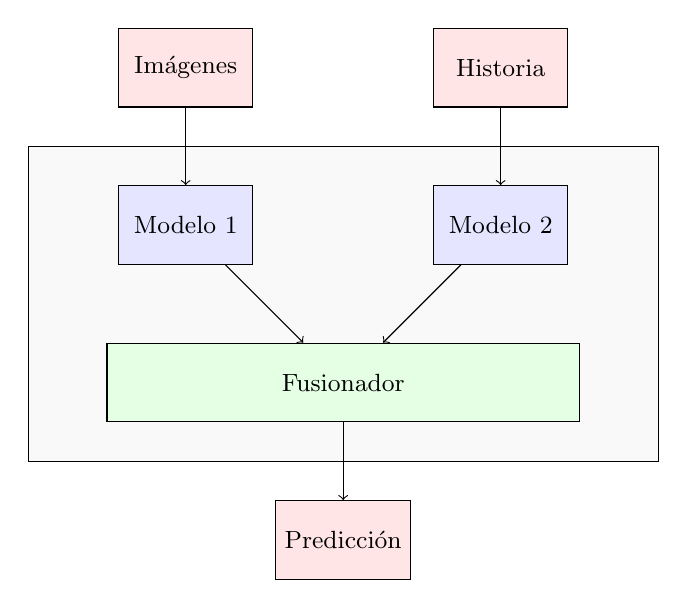
\begin{tikzpicture}[
every node/.style={font=\small},
datos/.style={draw, fill=red!10, minimum width=1.7cm, minimum height=1cm},
modelo/.style={draw, fill=blue!10, minimum width=1.7cm, minimum height=1cm},
fusionador/.style={draw, fill=green!10, minimum width=6cm, minimum height=1cm},
sistema/.style={draw, fill=gray!5}
]
% Datos
\node[datos] (datos1) at (-2,3) {Im\'agenes};
\node[datos] (datos2) at (2,3) {Historia};
% Sistema
\node[sistema, minimum width=8cm, minimum height=4cm] (sistema) at (0,0) {};
% Modelos
\node[modelo] (modelo1) at (-2,1) {Modelo 1};
\node[modelo] (modelo2) at (2,1) {Modelo 2};
% Fusionador
\node[fusionador] (fusionador) at (0,-1) {Fusionador};
% Salida
\node[datos] (resultado) at (0,-3) {Predicci\'on};
% Aristas
\draw[->] (datos1) to (modelo1);
\draw[->] (datos2) to (modelo2);
\draw[->] (modelo1) to (fusionador);
\draw[->] (modelo2) to (fusionador);
\draw[->] (fusionador) to (resultado);
\end{tikzpicture}
\end{center}
\end{frame}



\begin{frame}
\frametitle{Experimento 1}
\begin{itemize}
\item Los accuracies de ambos modelos 0.5 ambas clases
\item Fusionador de tipo OR
\item Correlaci\'on clase Positive de 0.95
\item Correlaci\'on clase Negative de -0.95
\end{itemize}
\vspace{3mm}
Se asignan distintos tamaños en cada dataset y para cada combinaci\'on se ejecuta 1000 veces y se reporta: \\
\vspace{3mm}
\begin{itemize}
\item $P(PeorCaso \geq EvalReal)$
\end{itemize}
\end{frame}



\begin{frame}
\frametitle{Experimento 1}
\centering
\includegraphics[height=0.8\paperheight]{Imgs/fijo_1000.png}
\end{frame}

\begin{frame}
\frametitle{Experimento 1}
La probabilidad se acerca r\'apidamente a 1 a medida que ambas cantidades de instancias aumentan. \\
\vspace{3mm}
Para el caso de un sistema con dos modelos, a tamaños no tan grandes, el peor caso usando datasets distintos provee casi la misma informaci\'on que con un solo dataset.
\end{frame}



\begin{frame}
\frametitle{Experimento 2}
\begin{itemize}
    \item Accuracies de ambos modelos aleatorias
    \item Fusionador aleatorio entre OR y AND
    \item Correlaci\'ones aleatorias v\'alidas para los accuracies
\end{itemize}
\vspace{3mm}
Los tamaños de ambos datasets tienen 10000 instancias por clase, se ejecuta 100000 veces y se reporta: \\
\vspace{3mm}
{\fontsize{17}{17}\selectfont
\begin{itemize}
\item $\frac{EvalReal}{PeorCaso}$
\end{itemize}
}
\end{frame}



\begin{frame}
\frametitle{Experimento 2}
\centering
\includegraphics[height=0.8\paperheight]{Imgs/random_100000_10000.png}
\end{frame}



\begin{frame}
\frametitle{Experimento 2}
El cociente entre ambos valores no suele pasar 1, siendo esto el resultado buscado. Incluso en los raros casos en los que si lo supera, no lo hace por un m\'argen muy grande. \\
\end{frame}